\newpage
\section{Экспериментальная часть}

Проведем тестирование и сравним алгоритмы по времени работы.

\subsection{Примеры работ}

На рисунках \ref{img:zero}, \ref{img:nef} и \ref{img:good} изображены примеры работ.

\begin{figure}[H]
    \centering
    
\includegraphics[scale=0.4]{zero_arg}
    \caption{Нет аргументов}
    \label{img:zero}
\end{figure}

\begin{figure}[H]
    \centering
    
\includegraphics[scale=0.4]{non_exist_file}
    \caption{Несуществующий файл}
    \label{img:nef}
\end{figure}

\begin{figure}[H]
    \centering
    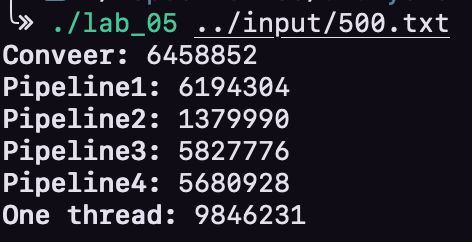
\includegraphics[scale=0.8]{good}
    \caption{Успешное выполнение}
    \label{img:good}
\end{figure}

\subsection{Результаты тестирования}

Для тестирования были использованы тесты в таблице \ref{table:test}.
Результаты продемонстрированы в таблице\ref{table:test-res}.

\begin{table}[H]
    \caption{Результаты тестирования}
    \label{table:test-res}
    \centering
    \begin{tabular}{|c|c|c|}
        \hline
        Первая матрца & Вторая матрица & Результат \\
        \hline
        1 2 & 1 2 & \ 7 10 \\
        3 4 & 3 4 & 15 22 \\
        \hline
        1 2 3 & 1 2 3 & \ 30\ \ 36\ \ 42 \\
        4 5 6 & 4 5 6 & \ 66\ \ 81\ \ 96 \\
        7 8 9 & 7 8 9 & 102 126 150 \\
        \hline
        1 2 3 & 1 & 14 \\
        4 5 6 & 2 & 32 \\
              & 3 & \\
        \hline
    \end{tabular}
\end{table}

Все тесты пройдены успешно.

\subsection{Замеры времени}

На рисунке \ref{img:graph} видно сравнение времени работы одного потока простив
конвейра на примере количества матриц от 100 до 1000.

\begin{figure}[H]
    \begin{tikzpicture}
        \begin{axis}[
            legend pos = north west,
            xlabel=Количество матриц,
            ylabel=микросекунды,
            grid = major,
            width = 0.8\paperwidth,
            height = 0.38\paperheight,
            line width = 1
        ]
            \legend{
                1 поток,
                Конвейер
            };

            \addplot coordinates {
                (100, 1979087)
                (200, 3938924)
                (300, 5899570)
                (400, 7890858)
                (500, 9846231)
                (600, 11803949)
                (700, 13777380)
                (800, 15747592)
                (900, 17697605)
                (1000, 19764128)
            };

            \addplot coordinates {
                (100, 1320171)
                (200, 2604349)
                (300, 3869893)
                (400, 5201684)
                (500, 6458852)
                (600, 7579206)
                (700, 8869803)
                (800, 10116102)
                (900, 11475725)
                (1000, 12852206)
            };
        \end{axis}
    \end{tikzpicture}
    \caption{Сравнение конвейра с 1 потоком}
    \label{img:graph}
\end{figure}

\subsection{Выводы}

Конвейерная реализация выигрывает у обычной примерно в да раза (рисунок \ref{img:graph}).
